\cleardoublepage
\setcounter{chapter}{6} %The counter for chapters should be set one less than 
                        %the actual chapter number, for example, {1} for 
                        %chapter 2, and {2} for chapter 3.
\setcounter{section}{7} %The counter for sections should be set to match the
                        %actual chapter number, for example, {2} for sections 
                        %in chapter, and {3} for sections in chapter 3. 
\chapter{Modifying WEBGUI}
\markboth{WEBGUI USERS' GUIDE}{MODIFYING WEBGUI}
\pagenumbering{arabic}
\setcounter{page}{59} %The counter for page numbers must be placed here in your
                     %chapter, following the \chapter and \markboth commands.
                     %It should always be the next available right-hand page.
                     %All chapters start on new rights. It will always be
                     %an odd number.  

\section{Introduction}
\label{sec:6-1}
This is an advanced section. Most users will never need to read this section. You do not need to read this 
section in order to use \f{WEBGUI} as a front end for your software. Everything you need to know about using
\f{WEBGUI} is contained in previous sections. Only read this section if you have special needs and would like
to customize or alter \f{WEBGUI}'s normal behavior.

\section{Overview}
\f{WEBGUI} is copyrighted by its author. It is ok to modify \f{WEBGUI} to your particular application
but please give credit to its author and note your modifications. This section helps explain how to modify \f{WEBGUI}. 
Since \f{WEBGUI} is basically a web server, modifying \f{WEBGUI} requires changing the default index.html file also.
Unlike ordinary web servers where this file is a separate file on the hard drive, \f{WEBGUI} contains
this file as data within its C code as an array of strings.

In the distribution of \f{WEBGUI}, we provide you with the file index.html as its own file and this section
explains how to modify it and place the contents back into webgui.c as data. Or alternatively this section
shows you how you can run webgui.c with an external index.html file. Additionally, \f{WEBGUI} displays
3 png images which are contained within the C code as an array of unsigned char.

Also to assist in customizing \f{WEBGUI} to your needs, this Chapter explains three more things; the 
communication between webgui.c and the web browser,  the private variables and functions of \f{WEBGUI}, 
and how WebGL works in both the web browser and webgui.c.

\section{index.html}
\label{sec:7-4}
The main task of \f{WEBGUI} is to be the front end for software and must receive input from the user and display output.
\f{WEBGUI} accomplishes this by utilizing a web page in a web browser. It creates a web page by mimicking a web server 
and then provides the file \textbf{index.html} to the client's web browser. On the client's side, the file \textbf{index.html} contains 
instructions to create a web page with buttons to receive input and display panes to show output. \textbf{index.html} contains
JavaScript code to allow the web page to be interactive and employs AJAX techniques. \textbf{index.html} also uses
HTML, CSS, and WebGL for formatting and display. On the server side, \textbf{webgui.c} mimics a web server, PHP processing,
and a MySQL database. \textbf{webgui.c} also interacts directly with software during runtime which 
is written in C or Fortran.

Whenever a web browser requests \textbf{index.html} it is created dynamically and then communicated as a string of characters. 
Within \textbf{webgui.c}, the file \textbf{index.html} is the concatenation of four string variables \textbf{webpageA}, \textbf{webpageB}, 
\textbf{webpageC}, and \textbf{webpageD}. Variable \textbf{webpageA} contains the beginning of \textbf{index.html} and the 
instructions to create the command buttons and input elements
to display and change parameters. \textbf{webpageB} contains instructions to create drop down menus to present options
for parameters. \textbf{webpageC} contains the overall layout of the web page and provides all the functionality. \textbf{webpageC}
is the majority of \textbf{index.html} and contains all the JavaScript, CSS, and WebGL. \textbf{webpageD} contains history information.
When you first load \textbf{index.html}, \textbf{webpageD} is mostly blank. If you reload your browser during your session,
then \textbf{webpageD} contains instructions to recreate the history of your session.

Every time a web browser requests \textbf{index.html}, \textbf{webpageA} is created fresh. Since \textbf{webpageA} contains
input elements to display parameters, \textbf{webpageA} must be updated at the time of a request to contain the current
parameter values. The portion \textbf{webpageB} is created once when \textbf{webinit} is called and never changed.
The portion \textbf{webpageC} is loaded once when \textbf{webstart} is called and never changed. Every time a web
browser requests \textbf{index.html}, \textbf{webpageD} is created fresh. Since \textbf{webpageD} contains the session 
history, \textbf{webpageD} must be updated to contain the current history. The web browser receives these four strings
consecutively and thinks it is receiving the one file \textbf{index.html}.

If you wish to change the appearance or function of the web page in the web browser, you must alter \textbf{index.html}.
To alter \textbf{index.html}, you must change the four pieces,  \textbf{webpageA}, \textbf{webpageB}, \textbf{webpageC}, 
and \textbf{webpageD}. To do this, you must alter the functions that build the pieces.
The piece \textbf{webpageA} is created in the function \textbf{updatewebpageA} within \textbf{webgui.c}.
In order for \textbf{webpageA} to create command buttons and work with parameters, it references the variables that 
contain information about commands and parameters. This information is contained in variables like \textbf{cmdn},
\textbf{cmda}, \textbf{cmdt} and \textbf{nn}, \textbf{na}, \textbf{nd}, etc. These variables are explained in Section \ref{sec:7-1}
below. 

The piece \textbf{webpageB} is created in the function \textbf{webinit}. The piece \textbf{webpageC} doesn't need to be created.
Instead it is loaded from either the hard drive or data within \textbf{webgui.c}. The next Section \ref{sec:7-2} explains this.
Finally, the piece \textbf{webpageD} is created in the function \textbf{updatewebpageD}. Section \ref{sec:4-2} explains how
\f{WEBGUI} can be used to display output only and not receive user input. That version of \textbf{index.html} uses a different
\textbf{webpageD} which gets created in the function \textbf{updatewebpageD2}.

Note that the best way to view \textbf{index.html} is to run \textbf{webgui.c} after linked to your software and then from your
web browser choose "View Source". (Google search "how to view a web page's source" if you don't know how to do this).
This will display the entire \textbf{index.html}. The beginning is \textbf{webpageA}. Following that is \textbf{webpageB} and 
\textbf{webpageC}. And the ending is \textbf{webpageD}. As a beginning point
of changing \f{WEBGUI}, you could save this file to your hard drive and start changing this file, reloading it, and seeing the consequence.
The best way to save \f{WEBGUI}'s webpage to a file is explained in Section \ref{sec:4-3}.

\section{External versus internal}
\subsection{indexC.html}
\label{sec:7-2}
The portion of \textbf{index.html} called \textbf{webpageC} is contained in the data variable \textbf{char indexhtml[x][y]} 
located at the end of \textbf{webgui.c}. This is an array of $x$ strings with each string having a maximum length of $y$. These
strings are the lines of the file \textbf{indexC.html} which resides on the hard drive. Since this data is within \textbf{webgui.c}, the
file \textbf{indexC.html} is not needed to run \f{WEBGUI}. The file \textbf{indexC.html} is only helpful if you wish to modify
\f{WEBGUI}.

If you wish to change the function or appearance of \f{WEBGUI}'s web page, then you can set the variable \textbf{load\_webpageC\_from\_file}
equal to 1. Afterward, make changes to the file \textbf{indexC.html}, and each time you quit and run \textbf{webgui.c}, it will load 
the new updated \textbf{indexC.html} from the hard drive. (You do not need to recompile \textbf{webgui.c} between trials). Once the web page 
appears and behaves as you like, you should place the file \textbf{indexC.html} within \textbf{webgui.c} as data. To do this,
you must convert each line into a string by placing quotation marks around it. And any quotation marks inside the line must have
a backslash added before. Any backslash needs an additional backslash before it. And care must be taken to convert the carriage
returns correctly. The easiest way to convert \textbf{indexC.html} into the array of strings \textbf{char indexhtml[x][y]} is to run
the program \textbf{convert2str.c}. It reads in \textbf{indexC.html} and writes the array of strings into \textbf{output.txt}. It also tells
you how many strings there are and the maximum length of these strings. Cut and paste the contents of \textbf{output.txt} into
\textbf{webgui.c}. Next, correct the value of \textbf{clines} in the function \textbf{updatewebpageC} to match \textbf{[x]}, the number of
strings. Finally, set the variable \textbf{load\_webpageC\_from\_file} equal to 0.

As an alternative to moving the contents of the file \textbf{indexC.html} within \textbf{webgui.c}, you can leave the variable
\textbf{load\_webpageC\_from\_file} equal to 1 and leave the file \textbf{indexC.html} in \textbf{webgui.c} local directory.

\subsection{png images}
\f{WEBGUI}'s web page displays 3 png images. A typical web server would have these images reside on the hard drive.
In the case of \textbf{webgui.c}, these images reside within the code of \textbf{webgui.c} as data. Specifically, they are the variables
\textbf{unsigned char folderpng[446]}, \textbf{unsigned char uppng[472]}, and \textbf{unsigned char filepng[402]}. In the web page,
these images appear when a user opens the drop down menu to select a file as shown in Figure \ref{fig:7-1}.

\begin{figure}[H]
\centering
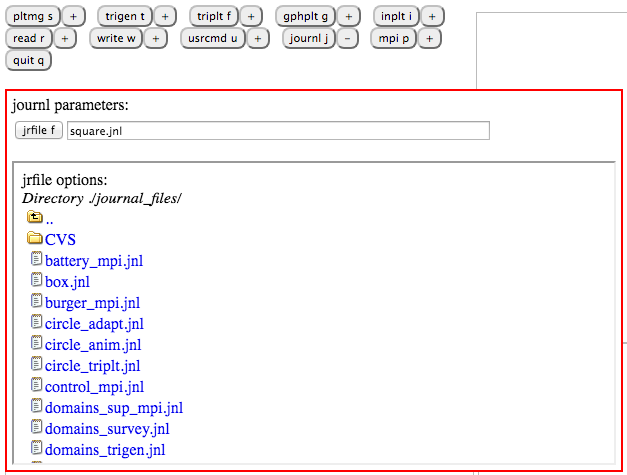
\includegraphics[width=0.75\textwidth]{pix/png.png}
\caption{User is selecting a file. Down the left side are png images. This figure shows WEBGUI interfaced with PLTMG.}
\label{fig:7-1}
\end{figure} 

In Figure \ref{fig:7-1}, the three png images named \textbf{up.png}, \textbf{folder.png}, \textbf{file.png} are shown to the left of the
blue words. These 3 files are provided with the distribution of \textbf{webgui.c} as external files. As explained above, they are not
needed to run \textbf{webgui.c} because their data is within \textbf{webgui.c}. These external files are provided in case a user
wishes to modify these images and/or make new ones.

If you wish to change the function or appearance of \f{WEBGUI}'s png images, then you can set the variable 
\textbf{load\_pngs\_from\_file} equal to 1. Afterward, make changes to the files \textbf{up.png}, \textbf{folder.png}, \textbf{file.png}, 
and each time you quit and run \textbf{webgui.c}, it will load 
the new updated files from the hard drive. (You do not need to recompile \textbf{webgui.c} between trials). Once the web page 
appears as you like, you should place the files within \textbf{webgui.c} as data. A png image 
file is just a sequence of byes (unsigned char). Therefore to place the data within \textbf{webgui.c}, just write these bytes as numbers 
in the declaration of the appropriate variable.

The easiest way to convert \textbf{up.png}, \textbf{folder.png}, \textbf{file.png} into an array of unsigned char is to run
the program \textbf{convert2int.c}. It reads in the png files and writes an array of unsigned char into \textbf{output.txt}. The usage for
\textbf{convert2int.c} is \textbf{convert2int source\_file}. After running \textbf{convert2int.c}, cut 
and paste the contents of \textbf{output.txt} into \textbf{webgui.c}. Finally, set the variable \textbf{load\_pngs\_from\_file} equal to 0.
 
As an alternative to moving the contents of \textbf{up.png}, \textbf{folder.png}, \textbf{file.png} within \textbf{webgui.c}, you can leave the variable
\textbf{load\_pngs\_from\_file} equal to 1 and leave the files \textbf{up.png}, \textbf{folder.png}, \textbf{file.png} in \textbf{webgui.c} local directory.

\section{Internal variables}
\label{sec:7-1}

\textbf{webgui.c} has many internal variables and functions. In this section, we will highlight the variables that
may be of interest to the reader wishing to modify \f{WEBGUI}. Important functions are highlighted in other sections when they
are relevant.

When software uses \textbf{webgui.c}, the first function that is called
is \textbf{webinit}. This function is explained in Section \ref{sec:2-1} and Section \ref{sec:3-1}. The purpose of calling \textbf{webinit}
is to add features to \f{WEBGUI}'s web page. Calling \textbf{webinit} can create command buttons and declare parameters. 
Declared parameters can be viewed and modified in the web page.

When \textbf{webgui.c} creates the web page, it references the declared parameters and requested command buttons. Information
about commands and parameters are stored in the following variables
\begin{verbatim}
static int cmdct, nct;
static const int maxnamelen=20, maxabbrlen=3, maxdeftlen=40;
static char **cmdn, **cmda, **cmdt;
static char **nn, **na, **nd, *nt;
static int **cmdp, *cmdpct, *cmdc;
static int *no, *nu, *nw, *ni;
\end{verbatim}

The above variables get initialized within the function call to \textbf{webinit}. All the variables that begin with the letter c reference
commands and all variables that begin with n reference parameters. Below are descriptions.\\
\textbf{const int maxnamelen=20, maxabbrlen=3, maxdeftlen=40} is the length of strings for name, abbreviation, and default values.\\
\textbf{int cmdct} is the quantity of commands.\\
\textbf{char** cmdn} is an array of strings equivalent to \textbf{char cmdn[cmdct][maxnamelen]} containing the full command names.\\
\textbf{char** cmda} is an array of strings equivalent to \textbf{char cmda[cmdct][maxabbrlen]} containing the abbreviated command names.\\
\textbf{char** cmdt} is an array of strings equivalent to \textbf{char cmdt[cmdct][maxnamelen]} containing the command types. Currently
this variable is initialized but unused.\\
\textbf{int* cmdpct} is an array equivalent to \textbf{int cmdpct[cmdct]} containing the quantities of parameters associated with each
command.\\
\textbf{int** cmdp} is an array equivalent to \textbf{int cmdp[cmdct][nct]} containing the indices of the parameters associated with each
command. Note that \textbf{nct} minus \textbf{cmdpct} elements are unused for each \textbf{cmdp[cmdct]}.\\
\textbf{int* cmdc} is an array equivalent to \textbf{int cmdc[cmdct]} containing 1 or -1 whether the respective command button is 
highlighted or not.\\
\textbf{int nct} is the quantity of parameters.\\
\textbf{char** nn} is an array of strings equivalent to \textbf{char nn[nct][maxnamelen]} containing the full parameter names.\\
\textbf{char** na} is an array of strings equivalent to \textbf{char na[nct][maxabbrlen]} containing the abbreviated parameter names.\\
\textbf{char** nd} is an array of strings equivalent to \textbf{char nd[nct][maxdeftlen]} containing the default parameter values. Note
that integer and real default values are stored as strings.\\
\textbf{char* nt} is an array of chars equivalent to \textbf{char nt[nct]} containing the parameter types (either i, r, s, l, or f).\\
\textbf{int* ni} is an array equivalent to \textbf{int ni[nct]} containing each parameter's index into their respective type's array.\\
\textbf{int* no} is an array equivalent to \textbf{int no[nct]} containing 1 or 0 whether the respective parameter has an options list.\\
\textbf{int* nu} is an array equivalent to \textbf{int nu[nct]} containing 1 or 0 whether the respective parameter is special. Ignore
this variable. Most likely your software will not use it.\\
\textbf{int* nw} is an array equivalent to \textbf{int nw[nct]} containing 1 or 0 whether the respective parameter is associated with 
a command or not.\\

Other important variables are
\begin{verbatim}
static const int maxlines = 100, maxhistory=100;
static int indexA = 0, indexB = 0;
static char *bufferA, *bufferB; //maintained as Fortran strings (space padded)
static char **history; //maintained as C strings (null terminated)

static char *webpageA, *webpageB, *webpageC, *webpageD;
static int load_webpageC_from_file = 1;
static int load_pngs_from_file = 1;

static float **colorsGL[3]={NULL,NULL,NULL};
static int ncolorGL[3]={0,0,0};
static float **triangles[3]={NULL,NULL,NULL};
static float **lines[3]={NULL,NULL,NULL};
static int indexT[3]={0,0,0}, indexL[3]={0,0,0};
static char *databuffer=NULL;
\end{verbatim}

The top group are explained in Section \ref{sec:7-3} below. The middle group are explained in Section \ref{sec:7-4} above.
The bottom group are explained in Section \ref{sec:7-5} below.

\section{Buffers and communication}
\label{sec:7-3}

\subsection{Overview}
The purpose of \f{WEBGUI} is to provide a front end for software. On behalf of software, \f{WEBGUI} receives input and displays output.
All input is in the form of command strings of maximum length 80. Output takes three forms. Output is either text, 2D images, 
or 3D objects. Output text is in the form of a string of maximum length 80. This section discusses input and output
strings and their communication. The following Sections \ref{sec:7-6} and \ref{sec:7-5} discuss the output of 2D images and 3D objects.

When a command button is pressed in the web browser of \f{WEBGUI}, the web page creates a command string and transmits
it to \f{webgui.c}. This command string waits in a command string buffer until the software requests it with a call to \textbf{webreadline}.
Software outputs text by calling \textbf{webwriteline(char* str)}. The outputted string waits in an output string buffer until the
web page requests it with an AJAX call. Therefore to facilitate input and output, buffers need to be maintained and strings need to
be transmitted between \f{webgui.c} (the web server) and the web page.

Software talks to \textbf{webgui.c} (directly via calls to \textbf{webreadline} and \textbf{webwriteline}), and \textbf{webgui.c} (the web server) 
talks to the web browser (via sockets and AJAX). All communication between a web browser and a web server (\textbf{webgui.c}) must be initiated 
by the web browser. And, all a web browser knows to do is request a URL. Whenever the web browser has a command string to pass on to the 
web server, the browser makes an AJAX request to the URL = http://localhost:15000/writeline.php?cmd='STR' where STR is replaced by the
command string of maximum length 80. And localhost:15000 is replaced by the host's ip address and listening port. In order for the 
web browser to receive output text from the web server, it continually asks if any text is available by making an AJAX request every half
second to URL = http://localhost:15000/readline.php . Each time, the web server responds with either an empty string, or a string of length 80. 
Every string that the web browser receives from readline.php, is displayed in the output text display pane with an appended html carriage return 
($<$br$>$).

\begin{verbatim}
static const int maxlines = 100, maxhistory=100;
static int indexA = 0, indexB = 0;
static char *bufferA, *bufferB; //maintained as Fortran strings (space padded)
static char **history; //maintained as C strings (null terminated)
\end{verbatim}

Above are internal variables within \textbf{webgui.c}.
Buffer B contains outputted text from the software. And buffer A contains command strings from the web browser. Each buffer
is an array of strings equivalent to \textbf{char buffer[maxlines][80]}. The variables \textbf{indexA} and \textbf{indexB}
track how many strings are in each queue. The software reads strings from bufferA and afterward they are removed from the queue.
The web browser reads strings from bufferB and afterward they are removed from the queue. A record of all strings is maintained
in a third array of strings named \textbf{char history[maxhistory][90]}. This is required in case the user refreshes the web browser.
If the web browser is reloaded and a new \textbf{index.html} is requested, then the web server must write the history of all previous commands 
and outputted text in the web page's output text display pane.

\subsection{Communication protocall}

The web browser and \textbf{webgui.c} (web server) pass strings back and forth. Every time a user
clicks a command button, the web browser sends a command string to the web server. Whenever a user closes a parameter drop
down menu after changing a parameter, the web browser sends a special capital letter command string (explained in Section \ref{sec:3-4}.)
Every time software has text to output, it calls \textbf{webwriteline} and the outputted string gets transmitted to the web browser.

In addition to the above three uses of strings, sometimes the web server needs to give the web browser special instructions. And sometimes
the web browser needs to give the web server special instructions. Whenever the web server needs to give the web browser a special
instruction, it places a number sign before the string. Below is an example.
\begin{verbatim}
#update,a=2,b=3.5,c=1
\end{verbatim}
Normally, the web browser assumes a received string is output text and displays it in the output text display pane. Whenever
the web browser sees a string that begins with a number sign, it doesn't display it. Instead it interprets it as a special instruction.
The web page's JavaScript function \textbf{processcmd(str)} (found in \textbf{indexC.html}) processes all special instructions.
The example above instructs the web browser to update (change) the value of parameters \textbf{a, b, c} to 2, 3.5, and 1 respectively.
Other special instructions are \textbf{image, webgl2, button, pause, start, unhide, lock, update, files}. The first two, instruct the 
web browser to request a waiting 2D image or 3D object. The next two highlight a command button and ask the user to click a
continue button. The last one, lists files on the web server's hard drive.

The web browser assumes that each received string is length 80. 
If a special instruction requires a longer string, it prefaces a string with a 
number sign followed by a number to indicate the number of length 80s it requires. For example
\begin{verbatim}
#3#update,key1=value1,key2=value2,etc
\end{verbatim}
The above example tells the web browser to expect that a string of length $240 = 80 \times 3$ is to follow. 

Whenever the web browser needs to give the web server a special instruction, it uses AJAX to contact the URL = http://
localhost:15000/callfunct.php?CMD=VAR where CMD is replaced with the desired special instruction and VAR is replaced with
the special instruction's variable(s). Within \textbf{webgui.c}, special instructions are processed within the routine 
\textbf{void *startlisten(void *arg)}. The special functions that are currently implemented are \textbf{continue, listfiles, release,
updateall, push, query, firewall, endian}.   

\section{2D Images}
\label{sec:7-6}

When software has an 2D image to output, it calls \textbf{websetcolors} and \textbf{webimagedisplay}. Afterward, \textbf{webgui.c}
notifies the web browser by sending a special instruction string
\begin{verbatim}
#image,WIDTH,HEIGHT,PANE
\end{verbatim}
where WIDTH and HEIGHT are replaced by the image's width and height. And PANE is replaced by the desired display pane.
Next, the web browser requests the image by requesting the resource \textbf{figure0.bmp}, \textbf{figure1.bmp}, or
\textbf{figure2.bmp} from the web server in a normal web browser - web server image request.

\section{3D Objects (WebGL)}
\label{sec:7-5}

When software has an 3D object to output, it calls \textbf{websetcolors, webframe, webline, webfill, webgldisplay}. Afterward, \textbf{webgui.c}
notifies the web browser by sending a special instruction string
\begin{verbatim}
#webgl2,PANE
\end{verbatim}
where PANE is replaced by the desired display pane.
Next, the web browser requests the 3D object by requesting the resource \textbf{data0.gpu}, \textbf{data1.gpu}, or
\textbf{data2.gpu} from the web server in a normal web browser - web server file request.

The "file" \textbf{dataX.gpu} is a binary data block. This block of memory is created in \textbf{webgui.c}'s function 
\textbf{int updatedatabuffer3(int x, int endian)}, then transmitted, then the memory is freed.
This "file" can be thought of as a sequence of numbers further divided into 3 sections; header, vertices, colors.

The first 80 bytes of \textbf{dataX.gpu} is the header which indicates the layout and length of the next two sections (vertices and colors).
The header is a sequence of 20 integers (4 bytes each). The first integer is the number of triangles
to draw in frame 5. The next integer is the number of lines to draw in frame 5.
The next 3 thru 10 integers are the number of triangles then lines for frames 3, 2, 4, 1 respectively. 
Integers 11 thru 20 are the numbers of triangles and lines declaring color information for frames 5, 3, 2, 4, 1 respectively.

Following the 20 integers (header section) is a sequence of 4 byte single precision floating point numbers. First come all the coordinates of the vertices for describing 
the triangles for frame 5. Each triangle is described by a sequence of 9 floating point numbers $(x1,y1,z1), (x2,y2,z2), (x3,y3,z3)$. 
Note that 1 triangle is 3 vertices is 9 coordinates.
Next come the coordinates of the vertices describing the lines for frame 5. Each line is described by a sequence of 6 floating point numbers,
$(x1,y1,z1), (x2,y2,z2)$.
Then triangles for frame 3, then lines frame 3, etc. Then frame 2, 4, 1.
 
Following the many coordinate floating point numbers (vertices section) is a sequence of 1 byte unsigned chars.
Each vertex has its own color and colors are 3 bytes, one unsigned char for each red, green, blue. Thus, if there 
are 10 triangles for frame 5 that require color declaration, then 90 unsigned chars are needed to describe the associated colors.
For example, a triangle's coordinates are 36 bytes as 9 floating point numbers, $(x1,y1,z1), (x2,y2,z2), (x3,y3,z3)$ 
and if that triangle declares colors then 9 bytes are needed as 9 unsigned chars, $(R1,G1,B1), (R2,G2,B2), (R3,G3,B3)$.

Therefore if \textbf{data[0]} is the first integer in \textbf{dataX.gpu} and \textbf{data[1]} is the second integer, then the size of \textbf{dataX.gpu}
in bytes equals the sum of the sizes of its three sections, (header) + (vertices) + (colors) which equals\\ 
$$\bigg(80\bigg) + \bigg(36 \sum_{k=0}^{4}data[2k] + 24 \sum_{k=0}^{4}data[2k +1]\bigg) + \bigg(9 \sum_{k=5}^{9}data[2k] + 6 \sum_{k=5}^{9}data[2k +1]\bigg).$$
This block of data is communicated to the web browser from
the web server. Then the web browser transmits this block of data (unaltered) into the client's GPU to display as WebGL.

For a given frame, usually the number of objects that declare colors (in colors section) is the same as the number of objects to 
be drawn (in vertices section) as in $data[k]=data[k+10]$ for $0\leq k \leq 9$. 
However, whenever all line colors are black for a particular frame then the associated $data[2k+1]$ for $5 \leq k \leq 9$ will equal 0
and the web browser and GPU know how to deal with that. (This saves bandwidth and memory.)

\subsection{Internal variables}

The "file" \textbf{dataX.gpu} only exists in \textbf{webgui.c}'s memory for a few seconds. When the software requests to display a 3D object by
calling \textbf{webgldisplay}, this temporary "file" is created in the variable \textbf{char *databuffer}, transmitted to the web browser, and then the 
memory is freed. This procedure is explained in Section \ref{sec:5-2}.

The permanent storage of a 3D object is stored in the following internal \textbf{webgui.c} variables:
\begin{verbatim}
static float **colorsGL[3]={NULL,NULL,NULL};
static int ncolorGL[3]={0,0,0};
static float **triangles[3]={NULL,NULL,NULL};
static float **lines[3]={NULL,NULL,NULL};
static int indexT[3]={0,0,0}, indexL[3]={0,0,0};
\end{verbatim}

Each time software calls \textbf{webline}, a new entry is added to \textbf{float **lines[3]}. In this triple array, \textbf{lines[0], lines[1], lines[2]}
are the lines for display panes 0, 1, 2 respectively. For display pane 0, \textbf{lines[0]} is equivalent to \textbf{lines[indexL[0]][8]} where
\textbf{indexL[0]} is the quantity of lines in display pane 0. Each line is represented by 8 floating point numbers. The first 6 are the 6 coordinates
of the 2 line segment endpoints, $(x0,y0,z0)$ and $(x1,y1,z1)$. The 7th float is the color (as an index reference to the color palette) and the 8th 
is the frame the line belongs to.

Each time software calls \textbf{webfill}, a new entry is added to \textbf{float **triangles[3]}. In this triple array, \textbf{triangles[0], triangles[1], 
triangles[2]} are the triangles for display panes 0, 1, 2 respectively. For display pane 0, \textbf{triangles[0]} is equivalent to 
\textbf{triangles[indexT[0]][11]} where \textbf{indexT[0]} is the quantity of triangles in display pane 0. Each triangle is represented by 11 floating point 
numbers. The first 9 are the 9 coordinates of the 3 triangle vertices, $(x0,y0,z0)$, $(x1,y1,z1)$, and $(x2,y2,z2)$. The 10th float is the color (as an index 
reference to the color palette) and the 11th is the frame the triangle belongs to.

The color palette is stored in the variables \textbf{float **colorsGL[3]} and \textbf{int ncolorGL[3]}. The color palette for display pane 0 is stored 
in the variable \textbf{colorsGL[0]} and is equivalent to \textbf{colorsGL[ncolorGL[0]][3]}. The variable \textbf{ncolorGL[0]} is the quantity of colors
in the palette of display pane 0, and each color is stored as 3 floating point numbers referring to the quantities of red, green, blue pigment.


